\begin{refsection}
    \renewcommand{\thefigure}{\arabic{figure}}

    \chapter[Sair da pirâmide e conhecer Além-Nilo: {\itshape ensino de história do Egito Antigo na Educação Básica}]{SAIR DA PIRÂMIDE E CONHECER ALÉM-NILO\\Ensino de história do Egito Antigo na Educação Básica\footnote{Inicialmente esse texto foi apresentado como comunicação intitulada ``Sair da pirâmide e conhecer além-Nilo: contribuições para o ensino de história do Egito Antigo para a educação básica'', no I Simpósio Internacional de Estudos em Egiptologia da Universidade de São Paulo (USP), realizado em setembro de 2019 nas dependências da USP.}}
    \label{chap:sairpiramide}
    
    \articleAuthor{Bruno Miranda Braga}
    {Doutorando em História pela Pontifícia Universidade Católica de São Paulo
    (PUC-SP). Atualmente bolsista do CNPq. Lattes ID: 9593.0970.5057.0247.
    ORCID: 0000-0001-7000-2456. E-mail: brunomirandahistor@hotmail.com.}

    \begin{galoResumo}
        \marginpar{
            \begin{flushleft}
                \tiny \sffamily
                Como referenciar?\\\fullcite{SelfBraga2021}\mybibexclude{SelfBraga2021},
                p. \pageref{chap:sairpiramide}--\pageref{chap:sairpiramideend},
                \journalPubDate{}
            \end{flushleft}
        } Exotismo, mistérios, encantos, pirâmides e faraós, são geralmente coisas que associamos em Educação básica, a aulas de Antiguidade --- oriente próximo --- Egito Antigo, como se esta civilização/país fosse algo distante, muito diferente se comparado a Antiguidade Clássica. O objetivo desse artigo é apresentar uma proposta de como está pensado o Egito Antigo no livro didático brasileiro, e destacar assim uma possibilidade de novos usos desses textos. De fato, o ensino de história do Egito Antigo no Brasil, segue uma cartilha já estabelecida na qual pouco se faz uso dessa ciência parceira, especializada no assunto que é a Egiptologia. Como a História, essa ciência está em construção, logo, fazer uso de seu discurso em sala de aula, significa fugir do grande rol de nome e datações históricas e focar na realização de uma história participativa, sendo a aula um elo no qual o conhecimento acadêmico expande sua aplicabilidade. Sair da pirâmide e conhecer o além-Nilo significa vislumbrar o Egito Antigo como era e como está atualmente.
    \end{galoResumo}
    
    \galoPalavrasChave{Ensino. Egito. Egiptologia. História.}
    
    \begin{otherlanguage}{english}
    
    \fakeChapterTwoLines
    {Leaving the pyramid and getting to know Beyond Nile}
    {teaching the History of ancient Egypt in Basic Education}

    \begin{galoResumo}[Abstract]
        Exoticism, mysteries, charms, pyramids, and pharaohs are things that we usually associate, in Basic Education, to Antiquity classes --- Near East --- Ancient Egypt, as if this civilization/country were something distant, very different compared to Classical Antiquity. This article aims to present a proposal of how Ancient Egypt is thought in the Brazilian textbook and thus highlight a possibility of new uses of these texts. Indeed, the teaching of History of Ancient Egypt in Brazil follows an already established standard which uses little of this partner science, specialized in the subject, that is Egyptology. Like History, this science is under construction, therefore making use of its speech in the classroom means escaping the great list of names and historical dates and focusing on performing a participatory history, the class being a link in which academic knowledge expands its applicability. Leaving the pyramid and getting to know Beyond Nile means envisioning Ancient Egypt as it was and how it is today.
    \end{galoResumo}
    
    \galoPalavrasChave[Keywords]{Teaching. Egypt. Egyptology. History.}
    \end{otherlanguage}

    \section{O Ensino de História Antiga na Educação Básica e a ``ciranda das civilizações''}

    Ainda hoje em nosso século XXI, o ensino de história na Educação Básica\footnote{Educação básica é aqui entendida a partir da proposta da Lei de Diretrizes e Bases. A Educação Básica, a partir da Lei de Diretrizes e Bases da Educação (LDB-9.394/96), passou a ser estruturada por etapas e modalidades de ensino, englobando a Educação Infantil, o Ensino Fundamental obrigatório de nove anos e o Ensino Médio.} no Brasil é um dos maiores desafios para o alunato e o professorado especializado ou não na área de História. Os alunos reclamam dos amplos contextos que a História redobra, os professores, tendem a afastar esses temas das realidades dos alunos, congelando e relegando a ``história ao passado, longínquo e remoto''.

    Tomando como base diferentes livros didáticos utilizados ao longo do território brasileiro, e devidamente credenciados e aprovados por comissões do Programa Nacional do Livro Didático (PNLD), esses livros em sua maioria, dividem a História antiga esquema da figura \ref{fig:hist-antiga-livro-did}.

    \begin{figure}[ht]%
        \centering%
        \caption{A História Antiga no Livro didático da Educação Básica}%
        \makebox[\textwidth][c]{\begin{tikzpicture}[%
            bluesty/.style={ellipse, draw=black, fill=galoblue!10},%
            greensty/.style={ellipse, draw=black, fill=galogreen!10},%
            yellowsty/.style={ellipse, draw=black, fill=galoyellow!10},%
        ]%
        % Nodes
            \node[greensty] (haeb) {História Antiga na Educação Básica};
            % 2nd row
            \matrix[row sep=0.3cm,column sep=0.5cm, ampersand replacement=\&] (sndrow) at ([yshift=-12mm]haeb.south) {
                \node[bluesty] (preh) {Pré-história}; \&
                \node[bluesty] (prciv) {Primeiras Civilizações}; \\
            };
            % 3rd row
            \matrix[row sep=0.3cm,column sep=0.5cm, nodes={align=center}, ampersand replacement=\&] (trdrow) at ([yshift=-12mm]sndrow.south) {
                \node[bluesty] (meso) {Mesopotâmia}; \&
                \node[yellowsty] (egyp) {Egito Antigo}; \&
                \node[bluesty] (crfenhe) {Cretenses, Fenícios e\\Hebreus}; \\
            };
            % 4th row
            \matrix[row sep=0.3cm,column sep=0.5cm, nodes={align=center}, ampersand replacement=\&] (fthrow) at ([yshift=-10mm]trdrow.south) {
                \node[bluesty] (per) {Persas}; \&
                \node[greensty] (grro) {Grécia e Roma}; \&
                \node[bluesty] (biz) {Império Bizantino}; \\
            };
            % 5th row
            \node[yellowsty] (fimia) at ([yshift=-12mm]fthrow.south) {1453 --- ``fim da Idade Antiga''};

            % arrows
            \draw (haeb) -- (preh);
            \draw (haeb) -- (prciv);
            \draw (preh) -- (prciv);
            \draw (prciv) -- (meso);
            \draw (egyp) -- (crfenhe);
            \draw (per) -- (grro);
            \draw (grro) -- (biz);
            \draw (biz) -- (fimia);

        \end{tikzpicture}}
        \caption*{Fonte: Autoria nossa para este estudo a partir da leitura de livros didáticos.}%
        \label{fig:hist-antiga-livro-did}%
    \end{figure}%

    De fato, ensinar História ainda hoje no Brasil não é uma tarefa fácil. A formação do licenciado embasada ainda no sistema 3 mais 1\footnote{A licenciatura no Brasil segue um sistema dos anos 80 do século XX, no qual o graduando para exercer o magistério passa 3 anos estudando questões relativas a uma área especifica do saber, e 1 ano com poucas e maus ministradas disciplinas voltadas para o ensino. Parece não haver conexão entre a pesquisa e o ensino. Porém, uma boa aula já induz uma pesquisa.}. A ampla precarização do sistema de ensino e a desvalorização docente também ressoam nesse processo.

    A história ensinada no Brasil parte da divisão preconcebida pela ``divisão tradicional da história'' em Antiga, Medieval, Moderna e Contemporânea. Para a Antiguidade, alvo deste texto, a educação básica parte de pressupostos tão prolixos e conteudistas que na maior parte das vezes, acaba mais confundindo os alunos que os ajudando. Penso que esse período histórico é o que é mais cheio de ``gavetas'' nas salas de aula do país.  

    Pela leitura do esquema, percebemos que a lógica é uma ``ciranda de civilizações'', uma sucessão de povos que fizeram parte desse período histórico. Essa ciranda em muito confunde nossos alunos. Parece ser que uma civilização sucede a outra de uma maneira destrutiva na qual a supremacia sempre é da civilização seguinte. É como se ao fim do estudo do Egito antigo, e ao iniciar as aulas de Creta, e Fenícia, os egípcios ``sumiram da história'' passaram a não existir mais. Tudo isso também se deve a uma recente área de estudos que é a Antiguidade no nosso país.

    \begin{quotation}
        A História Antiga, como conteúdo da disciplina do ensino de história, tem como característica ser exótica, distante e ao mesmo tempo atraente na sala de aula. É inegável que desperta curiosidade e admiração nos alunos, tanto do ensino fundamental quanto da graduação. As pesquisas em História Antiga iniciam no Brasil juntamente com a disciplina de História no âmbito universitário. O historiador Eurípides Simões de Paula fundou a primeira cadeira de História Antiga do país na Universidade de São Paulo na década de 1940 (CARVALHO; FUNARI, 2007). Mas seria somente nas últimas décadas do século XX que a área de História Antiga é marcada pelo aumento de sua produção científica, primeiro nas maiores e principais universidades do país e depois expandindo-se para as periféricas. \cite[p.~4]{SilvaAndGoncalves2015Ensino}. 
    \end{quotation}

    O exotismo ligado a História Antiga em sala de aula é inegável, o fascínio que ela desperta nos alunos idem. mas as relações, o feedback e a aplicabilidade dos conhecimentos desta parte da história, é quase nula, haja vista que é algo muito distante, e no qual ``após sucessivas guerras e batalhas, uma única civilização sobreviveu.'' O estudo da história antiga no nosso país por muito tempo objetivou a formação moral dos indivíduos, através da erudição, do classicismo, ao molde europeu. ``Era, definitivamente, um ensino voltado para as elites, e ainda hoje pode-se observar resquícios desse pensamento. Um primeiro ponto que precisa ser abordado sobre o ensino de história antiga na escola é que ela não é uma disciplina autônoma, mas sim, um conteúdo que pertence à disciplina de História Geral''.

    \begin{quotation}
        Nesse sentido o que se nota, na prática da sala de aula, é uma condensação da antiguidade clássica e oriental, já que o conteúdo deve obedecer a uma cronologia, sendo que a antiguidade clássica ainda recebe maior valorização do que a oriental na sala de aula.  

        A história antiga, dentre os conteúdos da disciplina de história, talvez seja aquela, que melhor possibilita ao aluno um encontro radical com o diferente, com a alteridade e com a pluralidade cultural. Claro que o termo Antiguidade condensa vários povos, religiões e línguas diferentes, em períodos de tempo longuíssimos, mas que na sala de aula, por vezes, são colocados todos como pertencentes a um mesmo quadro cultural. Nesse sentido a contribuição de outras áreas do conhecimento para o estudo da história antiga, como a arqueologia e a antropologia, é fundamental. \cite[p.~6]{SilvaAndGoncalves2015Ensino}. 
    \end{quotation}

    Eis o grande inimigo do ensino de História no Brasil, especialmente da História Antiga: um sistema cronológico e sucessivo. Como apontado anteriormente, no fluxograma, há uma sucessão, quase que sincronizada a respeito das civilizações da Antiguidade, sem haver relação nenhuma com o presente, nem com uma continuidade da anterior. Como sabemos, os estudos históricos partem de premissas diacrônicas, como propôs o historiador de Annales Fernand Braudel\footnote{Braudel redefiniu a noção de tempo histórico no qual partindo de suas proposições se estabeleceu: o tempo da o tempo breve, ou do acontecimento, o tempo a média duração, ou conjuntura, e a longa duração ou estrutura. É importante destacar que nos moldes Braudelianos o tempo histórico de uma civilização só se encaixa no tempo da longa duração, pois seus fazeres, saberes perpassam e atingem até mesmo outras fases históricas, suas estruturas permanecem. Ler mais em: \fullcite{Braudel1990Historia}.}, nisso, ``para Braudel a história factual, ou o tempo curto, que é como ele considera o fenômeno episódico, pode ser recomposta com documentos singulares, únicos, pois ela lida com aquilo que por essência é singular, elementos únicos porque são sempre singulares''.

    \begin{quotation}
        Mas podem existir vários documentos particulares falando de um só fato. Isso é até imprescindível, para seguir pela ``lógica da semelhança'' proposta por Marc Bloch. Nesse caso, trata-se de restituir os fatos na sua proximidade temporal e espacial, a sua sincronia e na sua diacronia, para se obter uma narrativa. Nesse âmbito, o da narrativa acontecimental, a história não aparece com muita lógica, a explicação avança pouco além da mera apresentação das causas simples que alinham um acontecimento ao outro, o que decorre mais da proximidade temporal e espacial entre os eventos do que de uma explicação de conjunto. O acontecimento é o limite, e no seu limite não existe explicação, aí prevalece o acaso, aquilo que não tem causa. \cite[p.~109]{Ribeiro2009Sincronia}.
    \end{quotation}

    E ainda hoje, o ensino de História Antiga no Brasil na Educação Básica segue essa lógica de ``ciranda das civilizações'' e isso torna-se prejudicial ao ensino pois se cria uma lógica ideal na qual uma civilização some, deixa de existir em detrimento do aparecimento de outra, há uma imposição de nomes e datas que mais confunde nosso alunato do que os ajuda. Em se tratando do ensino sobre o Egito, as dúvidas só se intensificam, pois além do mais é a única das civilizações que é acrescida onomasticamente com o predicativo ``antigo'' nos livros didáticos, levando a perceber um afastamento quase que completo por parte dos alunos.

    \section{O Egito Antigo no ensino: grandes nomes, grandes pirâmides, grandes dúvidas}

    Umas das questões que sempre aparecem em livros didáticos ao tratar do Egito é o nome ``EGITO ANTIGO''. Claro está que esta civilização ensinada e apresentada não é como, também não é nenhuma das outras vistas como estão hoje, e isso já é um problema, porém, não se lê em nenhum livro didático consultado no Brasil nomes como ``a Mesopotâmia Antiga'', ou ``A Pérsia Antiga''\footnote{Para este estudo, foram lidos e visitados aproximadamente 50 livros didáticos distribuídos e utilizados pelas cinco regiões do país. Não se trata de um estudo quantitativo, mas, qualitativo mesmo, no tocante ao trato com o ensino do Egito Antigo no Brasil.}. Essa tentação em apresentar algo tão longínquo é o primeiro grande problema para o ensino desta civilização, a partir do momento em que os estudos históricos partem sempre do presente para o passado, e no caso especifico do Egito, a ciência parceira, a Egiptologia é algo recente\footnote{Embora tenha se formado enquanto área do saber entre os séculos XIX e XX, é atualmente com o avanço das tecnologias, bem como dos grupos de pesquisa e formação de Egiptólogos que esta ciência vem avançando e se firmando mais como ramo de atuação e pesquisa.}. As duas descobertas primordiais para que a Egiptologia ganhasse respeito e se desenvolvesse: os hieróglifos, traduzidos por Jean-François Champollion por meio da Pedra de Roseta (século XIX) e a tumba de Tutancâmon, por Howard Carter (século XX), ainda hoje figuram como marco divisor do ensino da história egípcia.

    Ciro Flamarion \textcite[p.~7]{Cardoso2004Egito} nos mostra que:

    \begin{quotation}
        O Egito faraônico não somente representa o primeiro reino unificado historicamente conhecido, como também a mais longa experiência humana documentada de continuidade política e cultural. Mesmo não incluindo o período greco-romano --- embora os monarcas helenísticos e os imperadores de Roma tenham figurado como ``faraós'' em monumentos egípcios ---, a história do Antigo Egito se estende por uns dois e setecentos anos, de aproximadamente 3000 a.C. até 332 a.C.: como todas as datas relativas à civilização faraônica são anteriores à era cristã, eliminaremos doravante a menção ``antes de Cristo'', a não ser que por alguma razão seja necessária. Tal história conheceu, é verdade, fases de descentralização, anarquia e domínio estrangeiro, mas durante estes longos séculos o Egito constituiu uma mesma entidade política reconhecível.
    \end{quotation}

    A mais longa experiencia humana documentada de continuidade política e cultural. Eis o ponto central para melhor ensinarmos sobre o Egito faraônico na Educação básica: partir da premissa dos documentos que estão associados à sua imagem, e, a suas descobertas recentes. Assim entra em cena a ajuda bem-vinda da Egiptologia das suas técnicas e descobertas. O estudo desta ciência ainda está acontecendo, e assim como a história, se faz, refaz, a partir de novas descobertas e achados. Destacara isso para os alunos é evidenciar que a História é um construir/descontruir a partir de descobertas, é fazer da aula de história uma descoberta em construção, não incutir coisas herméticas e isoladas.  Essa atração pelo Egito antigo, se deve em parte, talvez às suas já mencionadas longevidade e continuidade. ``É um fenômeno fascinante o de uma civilização que, através de numerosas transformações, arrosta impávida várias dezenas de séculos sem perda das características essenciais que definem sua especificidade.'' \cite[p.~8]{Cardoso2004Egito}.

    Essas características essenciais a que Ciro Flamarion faz menção encaramos como aquilo que melhor esclarecia as peculiaridades do Egito sem deixar de fazer um link, uma proposta para com o dia a dia do nosso alunato. É interessante percebermos e apontamos também o que a Antiguidade egípcia nos legou, como fazemos quando tratamos de Grécia e Roma.\footnote{É muito comum o termo ``Antiguidade Clássica'' nos livros didáticos. O termo clássico por si só já engendra uma série de discussões que em sala de aula algumas vezes confunde a nós enquanto docentes, e aos nossos alunos. Clássico é comparado a erudito, ``fino'', civilizado, elegante, tradicional. E o pior: o clássico transmite a ideia de ``modelo a ser perpetuado''. Assim entendemos que a divisão entre Antiguidade e Antiguidade Clássica acarreta alguns problemas didáticos, que, o professor de História tende sempre corrigir, especialmente no Ensino Fundamental. Uma boa proposta seria o uso de Antiguidade Oriental e Antiguidade Ocidental.}

    \begin{quotation}
        Outra razão parece ser uma espécie de fascínio exótico e nostálgico exercido sobre o nosso mundo secularizado de hoje por alguns dos elementos culturais do Egito faraônico, em particular a realeza de caráter divino e a religião funerária tão elaborada, com sua obsessão milenar pelo renascer, pela imortalidade. 

        [\dots] É realmente fascinante tal mistura de convenção e naturalismo, a coexistência, que podemos seguir ao longo de milênios, de solenes cerimônias religiosas e monárquicas com cenas de felicidade doméstica, trabalho agrícola e artesanal, esportes e jogos --- enfim, mil detalhes da vida quotidiana de nobres e plebeus. \cite[p.~8]{Cardoso2004Egito}.
    \end{quotation}

    Esse fascínio para o Egito torna-se na educação básica algo além de prazenteiro, algo problemático à medida que se cria uma personificação para esta civilização que enfatiza apenas o mágico, o fascinante, o excêntrico. Assim, ao tratarmos desse conteúdo a partir da leitura e uso dos livros didáticos nos deparamos com uma experiência de ensino no qual ainda hoje pouco se relaciona com o cotidiano dos alunos, mas, que tem um leque de relações sem igual.  

    Dentro da divisão da história ocidental, é fascinante pensar o Egito como uma lógica de organização que perdurou por bastante tempo em continua e relevante realidade histórica humana. Logo, pensar o Egito pelas nossas singularidades assume a função de perpetuar e apresentar no espaço-tempo da História Antiga um eixo cultural e político bem como um poder dinástico até então jamais visto. Desconstruir o exotismo a excentricidade do Egito é apresentar como naqueles tempos uma sociedade se organizou e conquistou com ambivalência uma porção geográfica do crescente fértil a suas posses. Mas também é muito relevante apresentar as particularidades e ambiguidades da vida simples, fora das pirâmides de Gizé. Sistematicamente, no ensino básico as aulas de Egito se dividem no temário exposto na figura \ref{fig:ant-egit}.

    \begin{figure}[ht]%
        \centering%
        \caption{O Antigo Egito nos livros didáticos}%
        \makebox[\textwidth][c]{\begin{tikzpicture}
            % Nodes
            \node[draw, rounded rectangle, align=center, minimum width=80mm] (eaum) {Egito Antigo 01\\``Uma dádiva do Nilo''};
            \node[align=left, anchor=north west] (txtumgeo) at (eaum.south west) {Geografia do Egito Antigo};
            \node[align=left, anchor=north west] (txtumdh) at (txtumgeo.south west) {Divisão da História Egípcia};
            \node[align=left, anchor=north west] (anteg) at (txtumdh.south west) {\textbf{Antigo Império} (3200 a.C.--2100 a.C.)\\Pirâmides};
            \node[align=left, anchor=north west] (medeg) at (anteg.south west) {\textbf{Médio Império} (2100 a.C.--1580 a.C.)\\Expansão territorial\\Invasões hiscas};
            \node[align=left, anchor=north west] (noveg) at (medeg.south west) {\textbf{Novo Império} (1580 a.C.--715 a.C.)\\``Derrocada e conquista''\\``Fim do Egito''};

            \node[draw, rounded rectangle, align=center, minimum width=80mm, anchor=west] (eadois) at ([xshift=5mm]eaum.east) {Sociedade egípcia e\\o deus-sol o Faraó 02};
            \node[align=left, anchor=north west] (txtdhieso) at (eadois.south west) {Hierarquia social do Egito Antigo};
            \node[align=left, anchor=north west] (txtdtesc) at (txtdhieso.south west) {As três escritas: hierática, hieroglífica\\e demótica};
            \node[align=left, anchor=north west] (txtdgv) at (txtdtesc.south west) {Grão-vizir, sacerdotes, escribas e sábios};
            \node[align=left, anchor=north west] (txtfarao) at (txtdgv.south west) {O Faraó};

            \node[draw, rounded rectangle, align=center, minimum width=80mm] (eatres) at ([yshift=-37.49mm]eadois.south) {Religião no Egito Antigo};
            \node[align=left, anchor=north west] (txtttem) at ([xshift=6pt]eatres.south west) {Templos monumentais};
            \node[align=left, anchor=north west] (txttvid) at (txtttem.south west) {A vida após a Morte e o Livro dos Mortos};
            \node[align=left, anchor=north west] (txttpol) at (txttvid.south west) {Politeísmo e os deuses antropomórficos};
            

        \end{tikzpicture}}
        \caption*{Fonte: Elaborado pelo autor após leitura e consulta a livros didáticos.}%
        \label{fig:ant-egit}%
    \end{figure}%

    Destacamos que o conteúdo programático e curricular desenvolvido e apresentado nos livros didáticos, especialmente os aprovados pelo Programa Nacional do Livro Didático (PNLD)\footnote{O PNLD é destinado a avaliar e a disponibilizar obras didáticas, pedagógicas e literárias, entre outros materiais de apoio à prática educativa, de forma sistemática, regular e gratuita, às escolas públicas de educação básica das redes federal, estaduais, municipais e distrital e também às instituições de educação infantil comunitárias, confessionais ou filantrópicas sem fins lucrativos e conveniadas com o Poder Público. Segundo informações do Ministério da Educação (MEC), há um ciclo de escolhas e trocas de livros didáticos de acordo com as diferentes etapas da Educação Básica.} seguem em sua maior parte o sugerido pelos Parâmetros Curriculares Nacionais (PCNs)\footnote{Os PCNs versam sobre a estrutura do ensino fundamental. Dividido em ciclos, este documento direciona a ação educativa para as séries iniciais do fundamental (fundamental 01 --- do 1º ao 5º ano) até os anos finais do fundamental (fundamental 02 --- 6º ao 9º ano). Os PCNs foram promulgados em 1998. Para a área de História, o foco se dá a partir do fundamental 02 quando pela Lei de Diretrizes e bases da Educação Nacional, o ensino das disciplinas passa a ser de competência de um especialista na área, no caso, um professor com Licenciatura Plena em História.}, e pelas Orientações Curriculares para o Ensino Médio.\footnote{As Orientações Curriculares para o Ensino Médio, mediam o ensino básico final que são os três anos do Ensino Médio. Foram promulgados e renovados em 2006, incorporando novas questões que se tornaram lei para o ensino quer seja de história, quer seja de outro componente curricular como o ensino de temáticas Afro Indígenas. Pensadas pelo viés da inter multi transdisciplinaridade, as orientações estão organizadas em formato de agrupamentos por área do conhecimento. História, juntamente com Geografia, Sociologia e Filosofia, integram as competências das Ciências Humanas e suas Tecnologias. Transita pelo legislativo e executivo uma possível reforma no Ensino Médio, vamos acompanhar essas discussões e seus próximos passos e suas possíveis alterações na estrutura curricular.}

    Como as outras áreas do conhecimento humano, a história se transforma ao longo do tempo. Norberto \textcite{Guarinello2013Historia} enfatiza que a nova História Antiga é uma das peças mais importantes dessa reformulação. Para esse autor, a História Antiga se limita a estudar os primórdios, as origens do Ocidente, se dedica assim a um trabalho de memória e produção de uma identidade. Recebeu este nome por estar didaticamente no início da divisão sequencial da História, seguida pelas Medieval, Moderna e Contemporânea. O grande questionamento levantado por Guarinello é a respeito da sequência de acontecimentos, que denominamos de ``ciranda das civilizações''. ``A História da Grécia não acabou quando Roma começou'', nos declara o autor, por isso, historiadores buscam novas unidades de estudo com o objetivo de romper as sequências históricas, devido a seu caráter anacrônico.\footnote{Ler mais sobre essa discussão das sequências de sucessão na História antiga em: \fullcite{Guarinello2013Historia}.} Assim sendo, chegaremos num importante passo que é o estabelecimento de relações a partir da compreensão da História Antiga não como ``começo da História'', mas como a história de uma parte especifica do planeta, que tem ainda hoje relação com nossa atualidade, e principalmente com a atualidade de nossos alunos. 

    O ensino de história antiga, e consequentemente de Egito antigo aparece em dois momentos distintos na Educação Básica: nos conteúdos do sexto ano do fundamental, e no primeiro ano do médio. Evidentemente há uma clara distinção de linguagens e temáticas que são delicadas há algumas faixas etárias.\footnote{A faixa etária básica do alunato do sexto ano do fundamental é entre 11--13 anos. Para o primeiro ano do médio a faixa transita entre 15-16 anos, sendo essa classificação meramente ilustrativa.}

    Pela leitura das listas acima, sobre o temário do Egito Antigo nos livros didáticos, vemos que há uma série bem representativa para esse conteúdo já estabelecido e pouco modificado: para a unidade 01 a famosa afirmação de Heródoto de Halicarnasso ``o Egito é uma dádiva do Nilo''\footnote{A frase, atribuída ao historiador e geógrafo grego Heródoto de Halicarnasso, foi dita aproximadamente no século V a. C. Ler mais em: \fullcite[]{Herodoto2016Euterpe}.} é figura presente em todos os livros consultados. Aliás, nas atividades e listas de exercícios sempre há uma questão do tipo: ``comente a frase: o Egito Antigo é uma dádiva do Nilo'', ou ``o que seria essa dádiva do Nilo?'' A primeira unidade enfatiza sempre a  geografia do Egito junto ao delta do Nilo, e as etapas com uma estrutura de ruptura total com a anterior; uma breve apresentação sobre as pirâmides de Gizé, as invasões dos hicsos e tudo coroado pelo ``fim do Egito Antigo'', suas derrotas e seu apogeu sucessivamente pelos assírios (670 a.C.), persas (525 a.C.), gregos (332 a.C.) e romanos (30 a.C.), sem sequer ``mostrar o Egito Novo''.\footnote{Durante uma aula desta unidade, um aluno de sexto de uma escola da Cidade de Manaus-AM, me questionou ``professor, então a partir de agora nós iremos ver o `Egito Novo', pois o Antigo já foi conquistado, ne?'' A partir da inocente questão levantada por esse aluno, questionei ainda mais até que ponto os alunos compreendem temporal/espacialmente o Egito. As relações sempre partem do passado, e por lá permanecem, como se após a conquista romana, o Egito sumisse da história, sem ter uma continuidade.}

    A segunda unidade sempre focaliza na administração pública. A figura do faraó como centro da vida chega a transcender todas as demais questões. Repleta de simbologias de poder espiritual e temporal, essa unidade mostra apenas um lado da sociedade egípcia, pois:

    \begin{quotation}
        Muitas ``Histórias do Egito'' são, na verdade, quase exclusivamente Histórias dos reis egípcios: suas dinastias, batalhas, conquistas, construções e outros feitos. Uma tal distorção é em parte o resultado do caráter predominante da documentação escrita e arqueológica disponível, a qual ilumina sobretudo a religião e a monarquia. \cite[p.~9]{Cardoso2004Egito}.
    \end{quotation}

    E isso mesmo com todas as descobertas de historiadores, egiptólogos e arqueólogos permanece como centro do ensino.  

    Finalizando os estudos sobre o Egito vem toda a carga simbólica que fora anunciada na primeira unidade: a religião. Totalmente cheia de imagens, símbolos e signos, esta unidade se insere como a mais empolgante por parte dos alunos: as crenças egípcias. As pirâmides retornam com seu conteúdo explicado densamente, aparecem também as mastabas e os hipogeus, como túmulos. A religião egípcia antiga assume o centro da discussão cultural, e passa a moldar a representação de uma civilização que produzira uma sociabilidade repleta de hierofanias e teofanias que o próprio filho dos deuses era seu governante. E isso gera um fascínio sem igual. O problema é limitar esse fascínio ao contexto trabalhado e mostrar relação com o dia a dia dos alunos hoje, e evitar crenças fantasiosas demais e sensacionalismos.\footnote{É cada vez mais crescente a produção cinematográfica, documentarista e propagandista que se utilizam de elementos do Egito faraônico para despertar um discurso que varia desde esplendor até um exotismo como se essa civilização nem pertencesse a nosso gênero humano. Há uma difusão demasiada de crenças que os egípcios tiveram poções e elixires da imortalidade, e que inclusive tiveram contato extraterrestre, o que acarreta ao professor uma maior desenvoltura para limitar essa abordagem e, não levar os alunos a falsas e loucas afirmações sobre essa civilização.}

    \section{Sair da pirâmide e ir além-Nilo: uma proposta para o ensino sobre o Egito Antigo}

    Pensar a História ensinada a partir da perspectiva da realidade dos alunos, é transformar numa perene descoberta e algo prazeroso. Sempre que nos motivamos a realizar uma pesquisa histórica seja o tema que for, sempre partimos de uma inquietação atual, de uma problemática que nos circunda. Por que o ensino de História, especialmente das primeiras civilizações tem que ser apresentadas num passado ``antigo'' e congelado, sem estabelecer nenhuma conexão com presente e a realidade dos alunos? ``A supremacia do Egito no Brasil foi novamente enfatizada através de uma comparação de suas influências com a influência da comunidade brasileira negra no século XVII, o Palmares. Livros escolares dedicam apenas em média meia página para Palmares e é geralmente um único parágrafo''. 

    \begin{quotation}
        Isto, apesar de Palmares ser herança nacional e seu líder, Zumbi, ser considerado oficialmente herói nacional. Em contraposição livros escolares dão atenção especial para o Egito Antigo, e em especial para o que são consideradas seus maiores feitios e lendas míticas: a construção das Pirâmides e outros monumentos, suas misteriosas religiões e seu sucesso em produzir lucros. Todos os livros de história para os estudantes de 11 anos (sexta série) têm um capítulo de dez páginas dedicadas a civilização egípcia. Livros escolares do ensino médio para estudantes de 16 anos também dedicam pelo menos um capítulo inteiro para o Egito (FUNARI, 2004). Com base nessa comparação nós supomos que a resistência negra é desta maneira, pelo menos vinte vezes menos relevante do que o Egito como matéria em um livro de ensino (FUNARI e CARVALHO, 2006). \cite{FunariAndCarvalho2015Palmares}.
    \end{quotation}

    De acordo com Funari \citeyear{FunariAndCarvalho2015Palmares}, Egito Antigo é o conteúdo mais estudado, lembrado e popular da disciplina história na educação básica. Esta Civilização carrega um lugar especial no ideário social \cite{Silva2014Sorriso}, não se pode desperceber que, apesar do Egito antigo cronologicamente distante de nós, sua cultura e estilo não fazem parte de nosso conhecimento e cotidiano atual. Temos vários exemplos da presença do modelo egípcio em nossa sociedade, como por exemplo: novelas como ``Os dez Mandamentos, que virou filmes e foi exibido nos cinemas nacionais, além de outros filmes famosos como Cleópatra e Múmias. Além disso temos os desenhos animados que abordam a temática sobre o Egito antigo, ou sempre tem algum episódio que trata sobre o assunto, então repensar o distanciamento do Egito em nossas aulas torna-se a primeira proposta para o ensino. Lembrando que a História não é uma ciência do passado, nem estuda o passado, porém é a `ciência dos homens no tempo.'{}'' \cite[p.~32]{Bloch2001Apologia}.

    Além das diferentes propostas que diferentes autores já fizeram sobre como ensinar história, pensamos em usar as descobertas da egiptologia em sala de aula. Diferente da história nesse quesito, a egiptologia é uma ciência de ``pesquisa de campo aberto'' ``campo in loco''\footnote{Entendemos como ``pesquisa de campo aberto'' ``in loco'' aquelas nas quais os pesquisadores se deslocam para o local de pesquisa de campo geralmente a céu aberto, com escavações, e uso de instrumentos peculiares a esse \textit{métier}. O campo de pesquisa da História, geralmente é/são arquivos e bibliotecas, museus e outros, algo mais ``fechado'' ``de gabinete''. Já a egiptologia está quase sempre ``fora'', no local coletando e embasando novas descobertas.} o que acarreta uma aproximação maior com o cotidiano, com a vivência do seu objeto de pesquisa.  

    Em dezembro de 2018, líamos em diferentes veículos de informação que uma equipe de pesquisadores descobriu Tumba de 4 mil anos é descoberta no Egito. O túmulo do sacerdote chamado "Wahtye" data da 5ª dinastia (entre 2.500 e 2.300 a. C), durante o reinado de Neferirkare. Essa descoberta muito próxima a nós apresenta nomes que não comuns a quem não se debruça a pesquisar sobre o Egito. Além da importância histórica é evidentemente turística, o uso das informações contidas nas fotografias e relato dos pesquisadores nos permite emergir num universo que temporalmente está distante de nós, porém se pensarmos pelo viés social, até que ponto somos tão diferentes, ou eles eram tão diferentes?  

    Sobre essa descoberta, que é uma das mais recentes é interessante destacarmos o que a equipe de especialistas considerou sobre, e, problematizarmos com nossos alunos.

    \begin{quotation}
        O túmulo de um sacerdote que remonta a mais de 4.400 anos foi descoberto em Saqqara, perto do Cairo, por uma missão arqueológica egípcia, anunciaram neste sábado (15) as autoridades do Egito. O túmulo, do sacerdote chamado "Wahtye", data da 5ª dinastia (entre 2.500 e 2.300 a.C), durante o reinado de Neferirkare, de acordo com o Ministério das Antiguidades egípcio. 

        As informações são da agência France Presse. 

        A tumba está "excepcionalmente bem preservada, colorida com esculturas no interior. Ela pertence a um sacerdote de alta patente", explicou o ministro das Antiguidades, Khaled el Enany, a uma multidão de convidados. 

        O túmulo contém "cenas mostrando o dono da tumba com sua mãe, sua esposa e sua família, bem como vários nichos com grandes estátuas coloridas do falecido e sua família", disse o ministério em um comunicado. (Confira mais fotos ao final da matéria). 

        Os nichos são 18 e as estátuas, 24, de acordo com a mesma fonte, que especifica ainda que a parte inferior da tumba contém 26 nichos menores. 

        Em novembro, no mesmo sítio arqueológico em Saqqara, as autoridades egípcias revelaram a descoberta de sete túmulos, incluindo quatro que datam de mais de 6.000 anos, pela mesma missão arqueológica egípcia. 

        \vspace{5mm}

        \noindent\textbf{Os arqueólogos descobriram besouros e gatos mumificados.}

        \noindent{}O sítio de Saqqara, ao sul do Cairo, é uma vasta necrópole que abriga em particular a famosa pirâmide de degraus do faraó Djoser, a primeira da era faraônica. 

        Este monumento, construído em torno de 2.700 a.C pelo arquiteto Imhotep, é considerado um dos monumentos mais antigos da superfície do globo.\footnote{Tumba de 4 mil anos é descoberta no Egito. Veja fotos. Disponível em: \url{https://g1.globo.com/mundo/noticia/2018/12/15/tumba-de-4-mil-anos-e-descoberta-no-egito.ghtml}. Acesso em set. 2019.}
    \end{quotation}

    Com a informação apresentada pela equipe de pesquisadores a imprensa mundial temos um leque de possibilidades para trabalhamos em classe: as relações familiares entre os egípcios, porque enterrados juntos toda uma família? A relação dos egípcios com os animais, também mumificados, dentre outras temáticas. Quando tomamos para a sala de aula as imagens apresentadas, as possibilidades só se ampliam.  

    Concordamos com Thais Rocha \textcite[p.~187]{Silva2014Sorriso}, quando esta nos diz que: 

    \begin{quotation}
        Mas o Egito não é parte apenas do mundo islâmico e oriental. Ele não é apenas parte do grupo das ``civilizações orientais'', mas foi incluído também no grupo das ``civilizações africanas''. Contudo, não basta dizer que o Egito está na África. É preciso saber como colocá-lo ali afim de não deformar um Frankenstein oriental para fazer um africano. O precursor do afrocentrismo egípcio, Cheikh Anta Diop (1923-1986) retomou uma discussão apresentada ainda em finais do século XIX sobre a diáspora negra e a origem da humanidade no continente africano. Diop afrmava que o Egito antigo era uma civilização negra (1974: xiv) e reiterava a origem negra da civilização, tirando-a da posição de receptora e devedora do mundo branco ``ocidental''. 
    \end{quotation}

    \begin{figure}[ht]%
        \centering%
        \caption{Cinegrafistas e visitantes visitam o túmulo da Purificação Real do Sacerdote durante o reinado do Rei Nefer Ir-Ka-Re, chamado "Wahtye"}%
        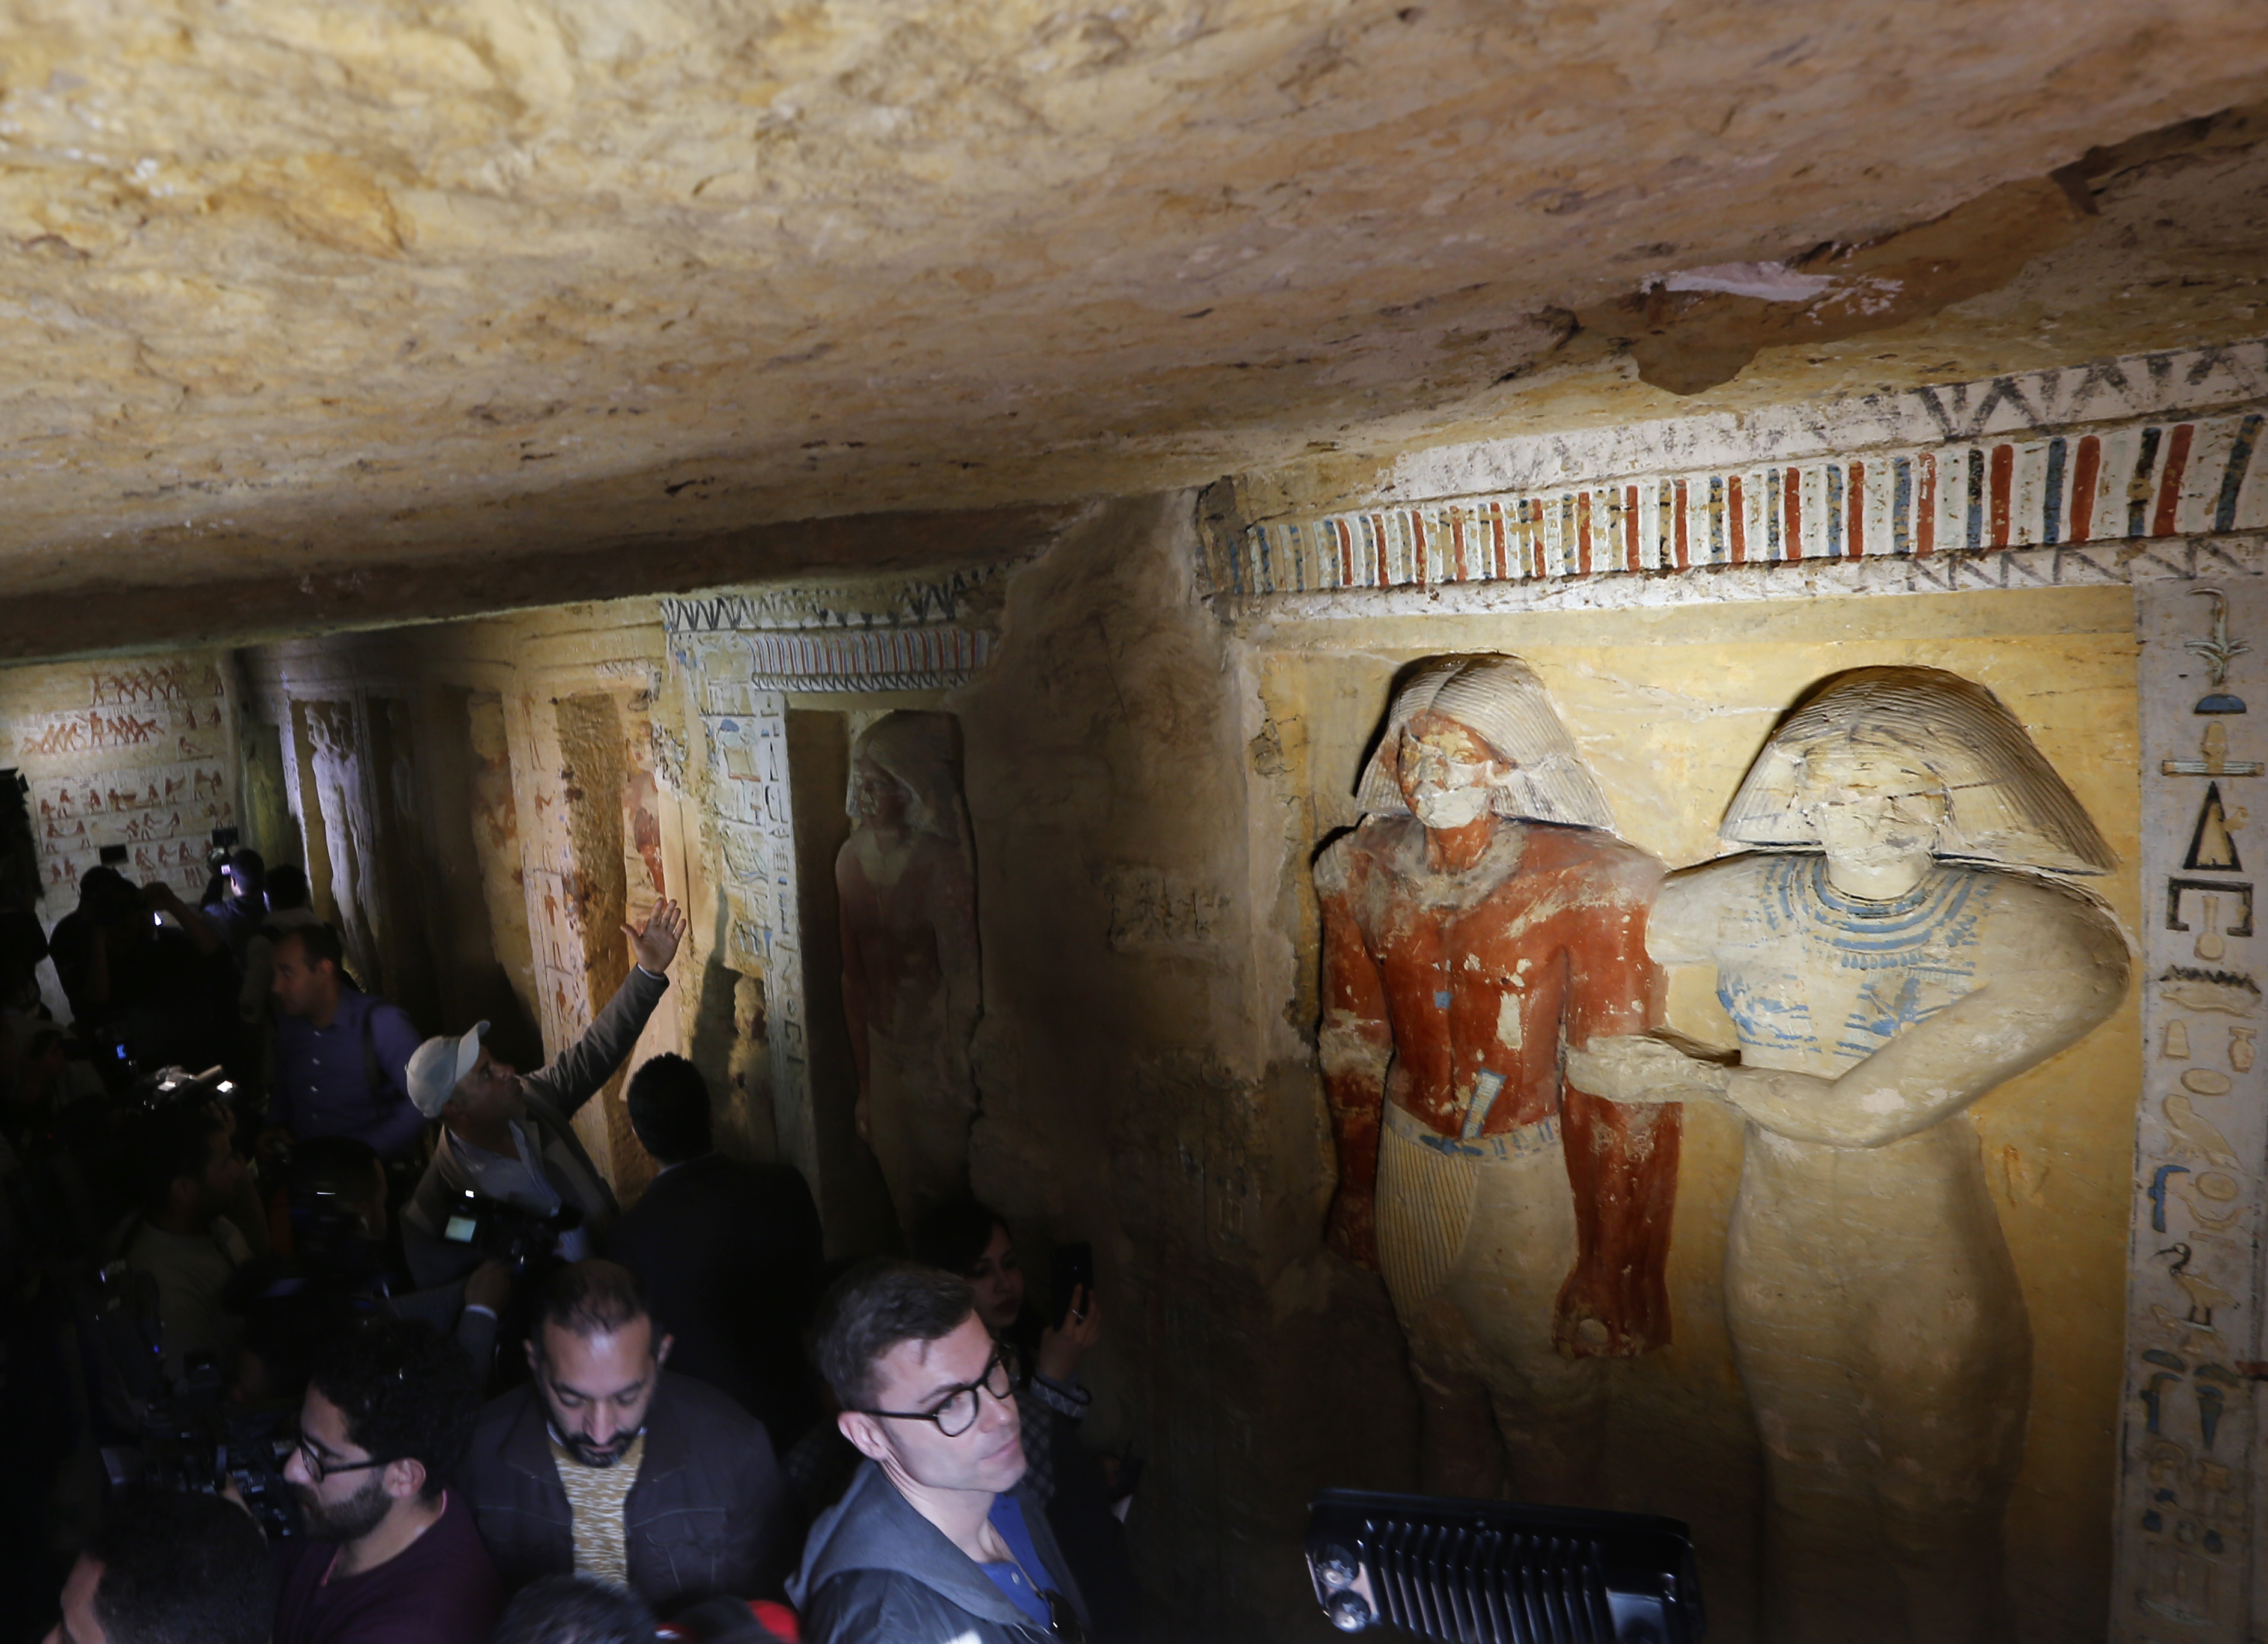
\includegraphics[width=.75\textwidth]{articles/16-sair-da-piramide-con/purif-real.jpg}%
        \caption*{Foto: AP Photo/Amr Nabil. Fonte: \url{https://g1.globo.com/mundo/noticia/2018/12/15/tumba-de-4-mil-anos-e-descoberta-no-egito.ghtml}.}%
        \label{fig:purif-real}%
    \end{figure}%

    \begin{figure}[ht]%
        \centering%
        \caption{Estátuas no túmulo recentemente descoberto da Purificação Real do Sacerdote durante o reinado do Rei Nefer Ir-Ka-Re, chamado "Wahtye"}%
        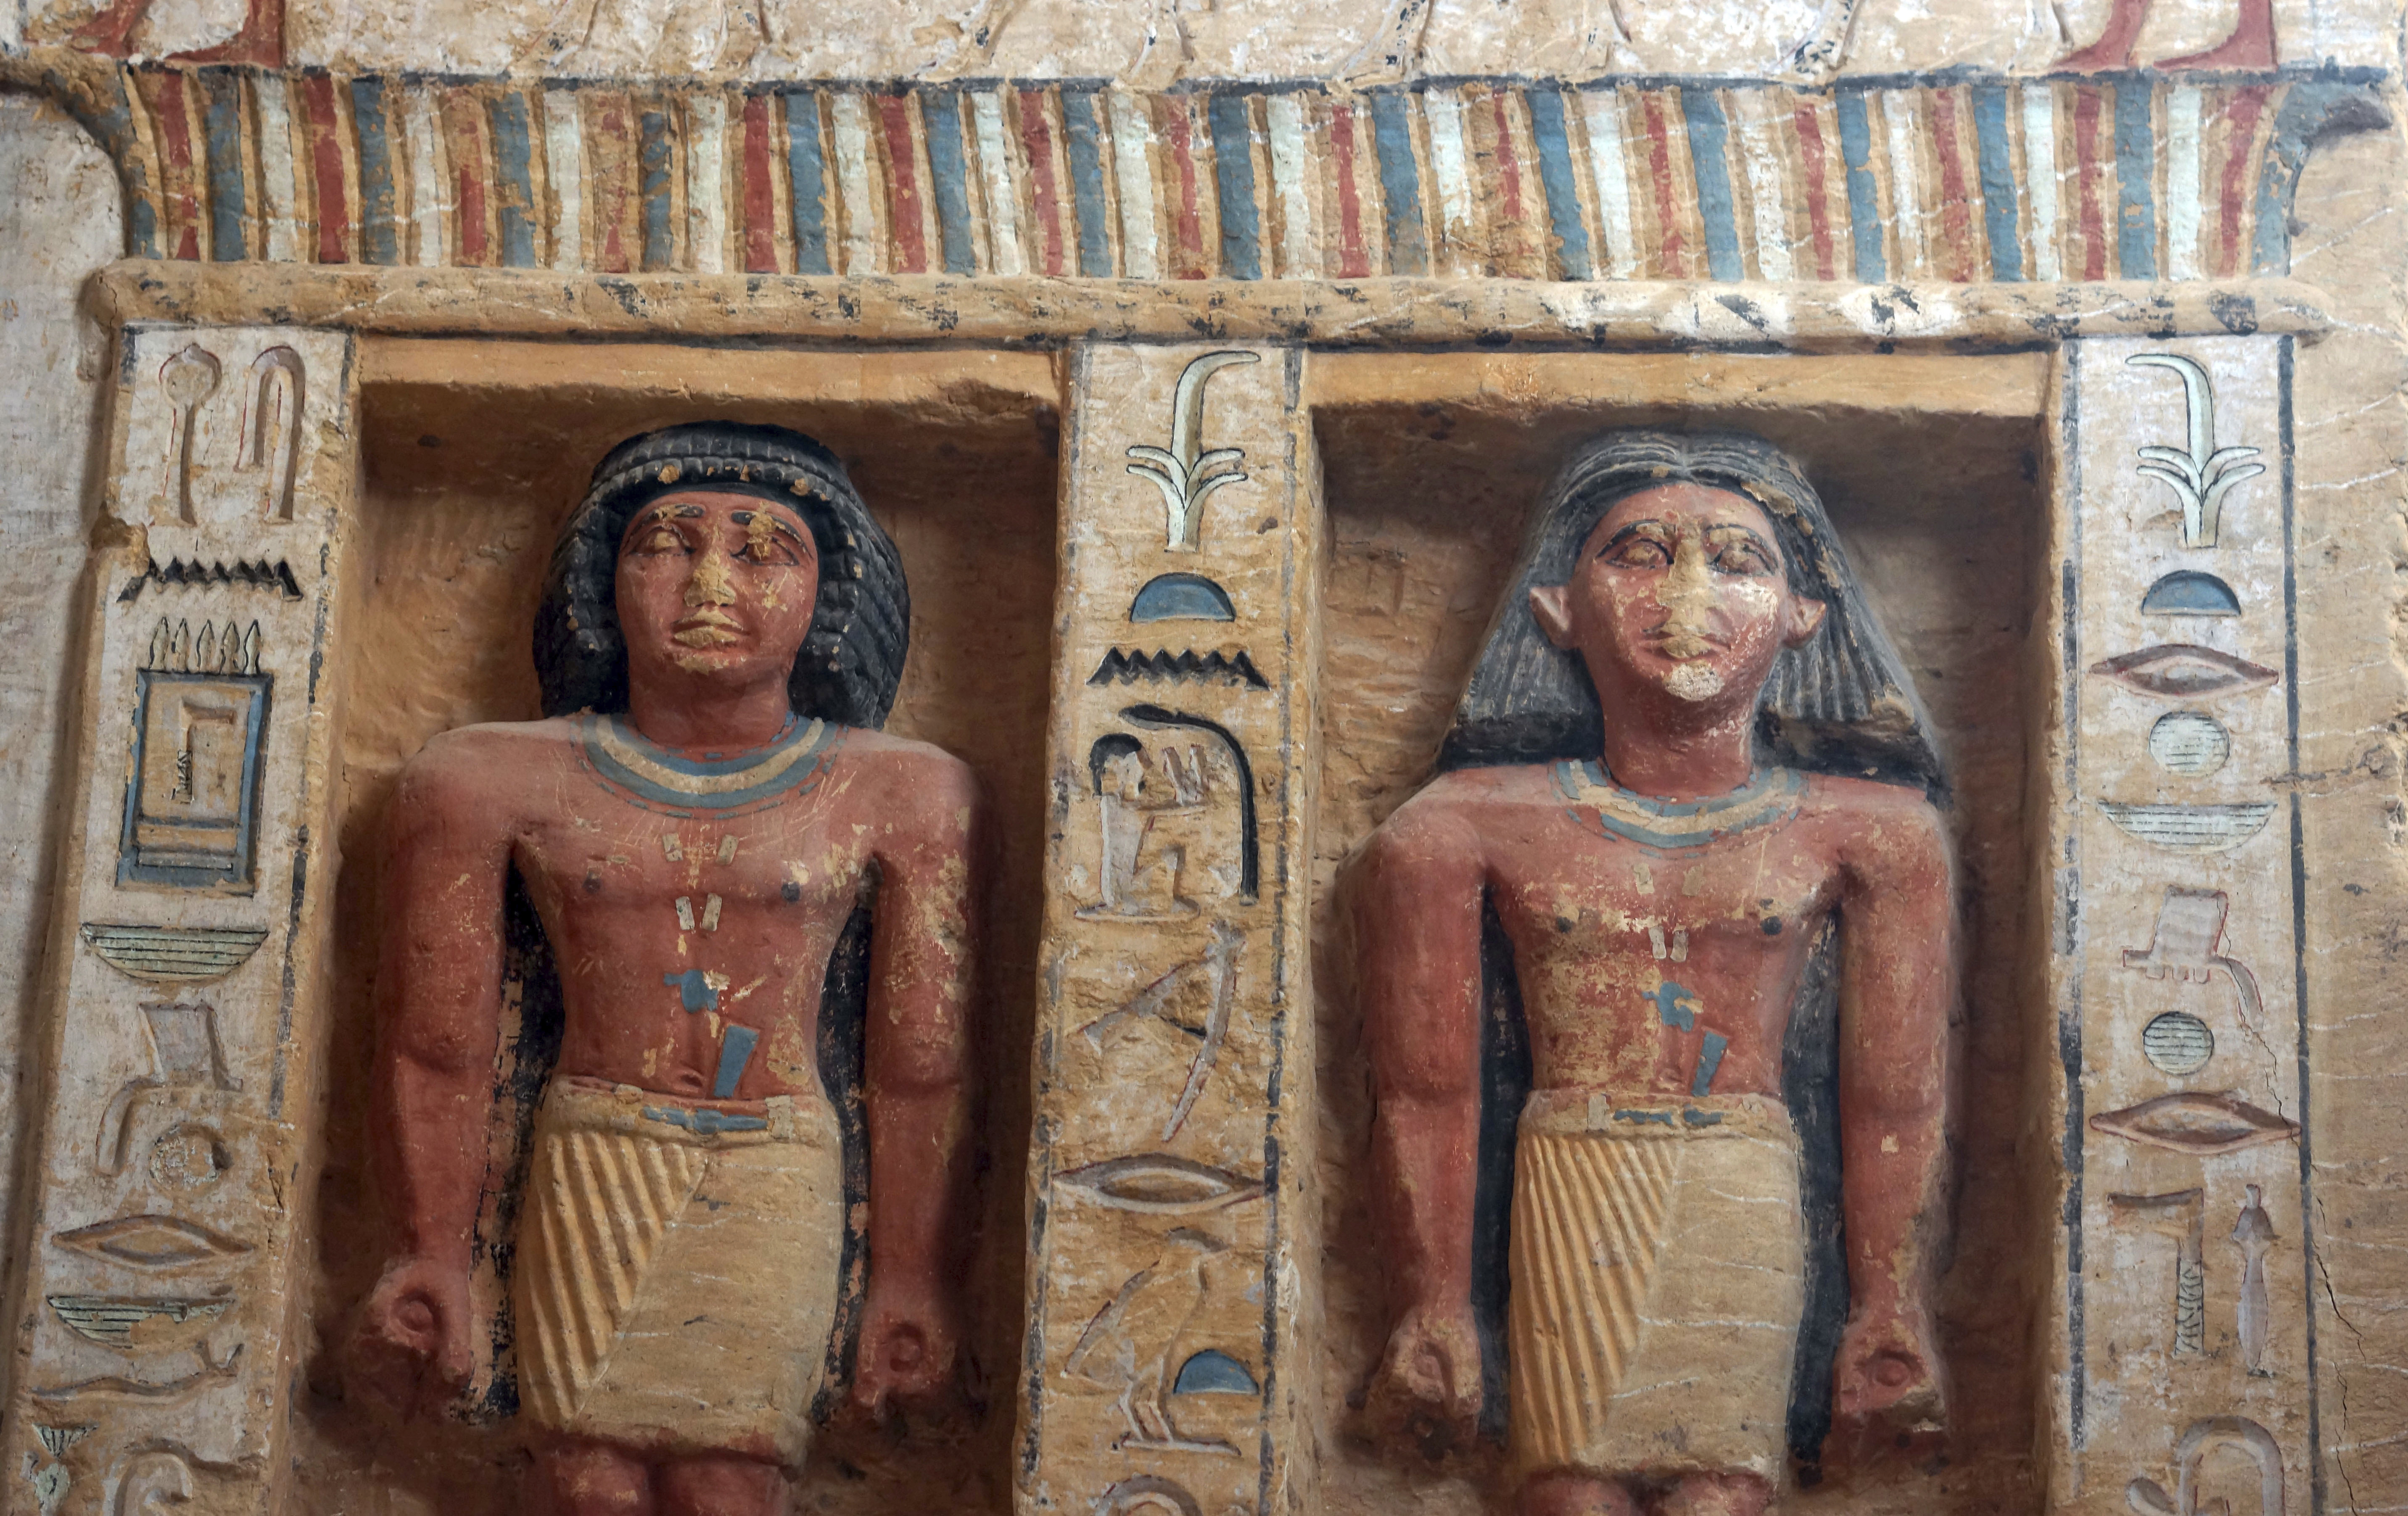
\includegraphics[width=.75\textwidth]{articles/16-sair-da-piramide-con/estatuas.jpg}%
        \caption*{Fonte: \url{https://g1.globo.com/mundo/noticia/2018/12/15/tumba-de-4-mil-anos-e-descoberta-no-egito.ghtml}.}%
        \label{fig:estatua-egypt}%
    \end{figure}%

    As duas imagens escolhidas dentre as demais (reproduzidas nas figuras \ref{fig:purif-real} e \ref{fig:estatua-egypt}) enfatizam pontos bem particuleres e recentes que pouco ainda são discutidos na educação básica: o primeiro grande ponto é a localização geográfica do Egito: o Egito está e sempre esteve no continente africano, logo, o esteriotipo hollywoodiano de ``egípcios de tez branca'' é algo para sempre levarmos a aula. Pelas fotografias acima, vemos uma representação colorizada de alguém da ``alta patente'' como noticiou o site. Sua tez não é branca. E sendo a tumba atribida a um lider, não seria genuino representá-lo com suas caracteristicas fisicas alteradas. Logo, os egipcios não eram ``tão branquinhos'' quanto se apresenta.

    \begin{quotation}
        Esse viés foi apropriado pelo movimento negro americano na década de 1960, comprometendo uma pesquisa arqueológica que insistia num Egito negro. Se por um lado ele mobilizou parte da comunidade científica para retirar o Egito do Oriente, expondo o orientalismo, foi inserido na África com uma série de problemas. A obra de Martin Bernal Black Athena, contribuiu para que os gregos saíssem do pedestal erigido pela academia dos séculos XVIII e XIX. Bernal se empenha em demonstrar que as construções em torno da ideia de desenvolvimento civilizacional ocorrem num sistema de cooperação, quase um ``orientalismo às avessas'' em que um Oriente (o dele) substitui os gregos no pedestal da civilização. \cite[p.~287]{Silva2014Sorriso}.
    \end{quotation}

    É importante assim destacar com os alunos que o Egito antigo foi uma grande dinastia com organização sociopolítica até então não vista no chamado ``Crescente Fértil'', que se diferenciou exponencialmente das demais civilizações por amplos fatores, especialmente pela divisão hierárquica concentrada na persona do Faraó e de seus tributários.     

    \section{Considerações finais}

    O desafio do ensino de História é sempre um guia em meio ao cotidiano escolar. Ensinar história é apresentar ao aluno um universo de possibilidades e antes de tudo relacionar! É mostrar aos alunos que cada povo, em cada período histórico vivencia as melhores experiencias de seu tempo.   

    O ensino da História Antiga é visto por muitos professores como a ``parte mais empolgante'' do ensino. De fato, há como mensuramos grande interesse por parte dos alunos nos assuntos que esse período histórico abarca: a ideia das lutas pérsicas, as conquistas Macedônicas, a mitologia greco-romana, e as pirâmides e faraós egípcios. O Egito Antigo carrega uma carga de interesse visual que os alunos já trazem consigo pela ampla difusão de uma egiptomania que seja a cultura pop, seja as mídias continuamente os apresentam. Nesse sentido, o professor também deve se apoderar do teor dessa mania e partir da premissa que os alunos sempre consideram algo sobre o Egito, e esse algo deve ser desmitificado, e mostrado como algo comum, não fora dos limites humanos.  

    O livro didático com sua postura reducionista acaba aludindo ideias simplistas sobre a civilização egípcia na qual ainda pouco se fala como está o Egito hoje. Não se estabelece uma conexão com o dia a dia, com o vivido por nossos alunos. Compete assim ao professor também a tarefa de relacionar, de estabelecer uma conexão entre o discurso do livro, a descobertas recentes da Egiptologia, e a realidade vivida por nossos alunos, isso parece ser algo difícil, mas não o é uma vez que a melhor maneira de ensinar história é sempre partimos de nosso presente para o passado, assim construirmos conhecimento!


    \nocite{Presse2018Tumba}

    \printbibliography[heading=subbibliography,notcategory=fullcited]

    \hfill Recebido em 6 abr. 2021.

    \hfill Aprovado em 16 abr. 2021.

    \label{chap:sairpiramideend}

\end{refsection}
